\documentclass[10pt,a4paper]{article}
\usepackage[margin=1.9cm]{geometry}
\usepackage[T1]{fontenc}
\usepackage{lmodern}
\usepackage{microtype}
\usepackage{amsmath,amssymb}
\usepackage{graphicx}
\usepackage{booktabs}
\usepackage{multirow}
\usepackage{array}
\usepackage[font=small,labelfont=bf,skip=3pt]{caption}
\usepackage[compact]{titlesec}
\usepackage{enumitem}
\usepackage[hidelinks]{hyperref}
\setlist{nosep,leftmargin=1.2em}
\titlespacing*{\section}{0pt}{6pt}{3pt}
\titlespacing*{\subsection}{0pt}{4pt}{2pt}
\setlength{\parskip}{2pt}
\setlength{\textfloatsep}{8pt}

\newcommand{\etaA}{\eta_A}
\newcommand{\etaB}{\eta_B}



\begin{document}
\begin{titlepage}
    \centering
    \vspace*{1cm}
    
    % Replace 'logo.png' with the path to your image file
    \includegraphics[width=0.5\textwidth]{logo.png} \\[1.5cm]
    
    {\Large Department of Electronic \& Telecommunication Engineering \\ 
    University of Moratuwa, Sri Lanka} \\[1cm]
    
    {\Large EN4554 Deep Learning for Vision} \\[1cm]
    
    {\Large \textbf{Assignment 1: LoRA finetuning and LLM tool-calling} \\[1cm]

    {\Large Manawadu D.N.  220380J} \\
    {\Large Nadha M.I.  220409J} \\[1cm]
    \small GitHub: \url{https://github.com/NadhaIrshad/EN4554-Deep-Learning-for-Vision-A01.git}}\\[1cm]

    {\Large Date: 16.10.2026} \\[1cm]
    
    \vfill
\end{titlepage}

\section{Central claim of the paper}
LoRA+~\cite{loraplus} argues that standard LoRA~\cite{lora}, which uses one learning rate for both adapter matrices
($\Delta W = BA$), cannot learn features efficiently in wide models. Setting $\etaB = \lambda\,\etaA$ with
$\lambda \gg 1$ fixes this and reports 1--2\% better accuracy and up to $\sim\!2\times$ faster fine-tuning at the
same cost.

\section{Concept translated, and the evidence for it in the paper}
\textbf{Concept: efficient feature learning requires $\etaB/\etaA \gg 1$.} Write the change in a LoRA layer's output
after one optimiser step as two linear terms: $\delta_A = B_{t-1}(A_t - A_{t-1})x$ (updating $A$) and
$\delta_B = (B_t - B_{t-1})A_{t-1}x$ (updating $B$). The paper calls training \emph{efficient} when both terms are
$\Theta(1)$, and shows that with $\etaA = \etaB$ this is impossible as width $n\to\infty$. With the standard
initialisation ($B_0 = 0$), $B$ is the matrix that is not updated efficiently, so the fix is
$\etaB/\etaA = \Theta(n)$. \textbf{Supporting evidence:} the $(\etaA, \etaB)$ test-accuracy heatmaps for
RoBERTa-base on GLUE and GPT-2 on MNLI/QQP (Figs.~3--4 of~\cite{loraplus}) have their optimum \emph{off the
diagonal}, at $\etaB > \etaA$, with the paper recommending $\lambda \approx 2^4$. The paper also notes that the gap
is larger on harder tasks and that $\etaA = \etaB$ is nearly optimal when little feature learning is needed (Llama-7b
on MNLI).

\section{Translated hypotheses}
For a small VLM fine-tuned with LoRA on visual question answering:
\begin{itemize}
  \item \textbf{H1 (optimum):} in an $(\etaA, \lambda)$ grid, the best cell has $\lambda > 1$ and beats a
        \emph{tuned} LoRA ($\lambda = 1$).
  \item \textbf{H2 (accuracy and speed):} tuned LoRA+ reaches higher test accuracy (H2a) and reaches LoRA's final
        validation loss or accuracy in fewer steps (H2b).
  \item \textbf{H3 (mechanism):} with $\lambda = 1$, $\delta_A$ and $\delta_B$ are strongly unbalanced, and LoRA+
        moves them towards balance.\footnote{Our project notebook originally predicted the opposite direction
        (LoRA+ raises $A$'s share of $\Delta W$). After the first results we re-read \S3 of~\cite{loraplus}, which
        identifies $B$ as the under-updated matrix, and restated H3. The weight-share measurement was not changed;
        the $\delta$ measurement was added afterwards to test the paper's mechanism directly. The restated
        hypothesis is still not supported (\S5). Full account: \texttt{part1/README.md}.}
  \item \textbf{H4 (harder task):} the LoRA+ gain is larger on an OCR-heavy task (TextVQA) and on harder question
        types.
  \item \textbf{Bonus, specific to VLMs:} a VLM mixes layers of very different width, unlike the LLMs the paper
        studies. The pixel-shuffle connector has fan-in $768\times16 = 12288$, against 576 (text) and 768 (vision).
        If the optimal ratio is $\Theta(\text{fan-in})$, a \emph{single global} $\lambda$ is wrong for a VLM, and
        a width-scaled $\lambda_\ell = \lambda_0\,n_\ell/576$ should do better. We also ask which tower,
        vision or language, carries (or suffers from) the LoRA+ effect.
\end{itemize}

\section{Experimental setup}
\textbf{Model.} SmolVLM-256M-Instruct~\cite{smolvlm} (SigLIP vision encoder, width 768; SmolLM2 decoder, width 576),
which is within the $\le$500M limit. Images use a single 512\,px tile (64 visual tokens; image splitting is off) to
keep runs short. LoRA has rank 8, $\alpha = 16$ and dropout 0.05, on every attention and MLP projection of both
towers: 3.8M trainable parameters (1.45\%). The vision$\to$text connector is \emph{not} adapted, except in the
connector experiment (Further experiment 1). The loss is on the assistant turn only.

\textbf{LoRA+.} Two AdamW parameter groups: \texttt{lora\_B} uses $\lambda\etaA$ and everything else $\etaA$.
Weight decay is 0, the schedule is linear with 5\% warm-up, gradients are clipped at 1.0, and training uses fp16
autocast with fp32 master weights. Batch size is 8 and training runs for 2 epochs (750 steps). Prompt:
\emph{``\{question\} Answer with a single word or short phrase.''}; decoding is greedy with at most 10 new tokens.

\textbf{Data (seed 42).} \emph{VQAv2}~\cite{vqav2}: \texttt{merve/vqav2-small} (21{,}435 questions from VQAv2
\emph{val}), with 3000 train / 300 val / 500 test questions. This subset stores a single consensus answer and no
image IDs, so the split is random by question and we report \textbf{exact-match} accuracy. \emph{TextVQA}~\cite{textvqa}:
\texttt{lmms-lab-encoder/textvqa} \emph{validation} (5000 questions), split \textbf{by image} into 3000 / 300 / 492
questions, using the standard VQA accuracy over the 10 annotator answers. TextVQA was chosen as the harder task: it
requires reading text in the image, so it needs more new visual features (H4).

\textbf{Protocol.} \emph{Selection} uses the val split only. Grid: VQAv2 $\etaA\in\{5\mathrm{e}{-5}, 1\mathrm{e}{-4},
2\mathrm{e}{-4}, 5\mathrm{e}{-4}\} \times \lambda\in\{1,4,16,32\}$; TextVQA $\{1,2,5,10\}\mathrm{e}{-4}\times\{1,4,16\}$.
The $\lambda=1$ column is an LR sweep for plain LoRA, so the baseline is tuned exactly as in the paper, and both
optima are interior to their grids. Grid runs are shorter than final runs (1500 examples, 1 epoch vs.\ 3000, 2
epochs); at full budget the val ranking of LoRA's $\eta$ on TextVQA is preserved (5e-4: 41.0 vs.\ 1e-4: 38.9).
\emph{Comparison:} tuned LoRA, tuned LoRA+, and LoRA+ with the paper's $\lambda=16$ at LoRA's $\eta$ (``drop-in''),
each with 3 training seeds (42/43/44), reported on the \emph{test} split. \emph{Claim-tied metrics:} the grid
optimum (H1); for speed (H2b), on both datasets, the number of seeds that reach 95\% of tuned LoRA's final val
accuracy and that reach its final val loss, with the median step (val accuracy is checked every $\approx$94
steps, val loss every $\approx$37); $\delta_A/\delta_B$, logged every 25 steps on a fixed batch of 4 val examples,
median over layers per tower (H3); and accuracy split by question type (H4). All runs used an RTX\,4090
($\approx$10\,min per 750-step run). Training uses fp16, not bf16, so it also runs on a Colab T4; we estimate
25--40\,min per run there, but have not measured it.

\section{Results and interpretation}
\begin{figure}[t]
  \centering
  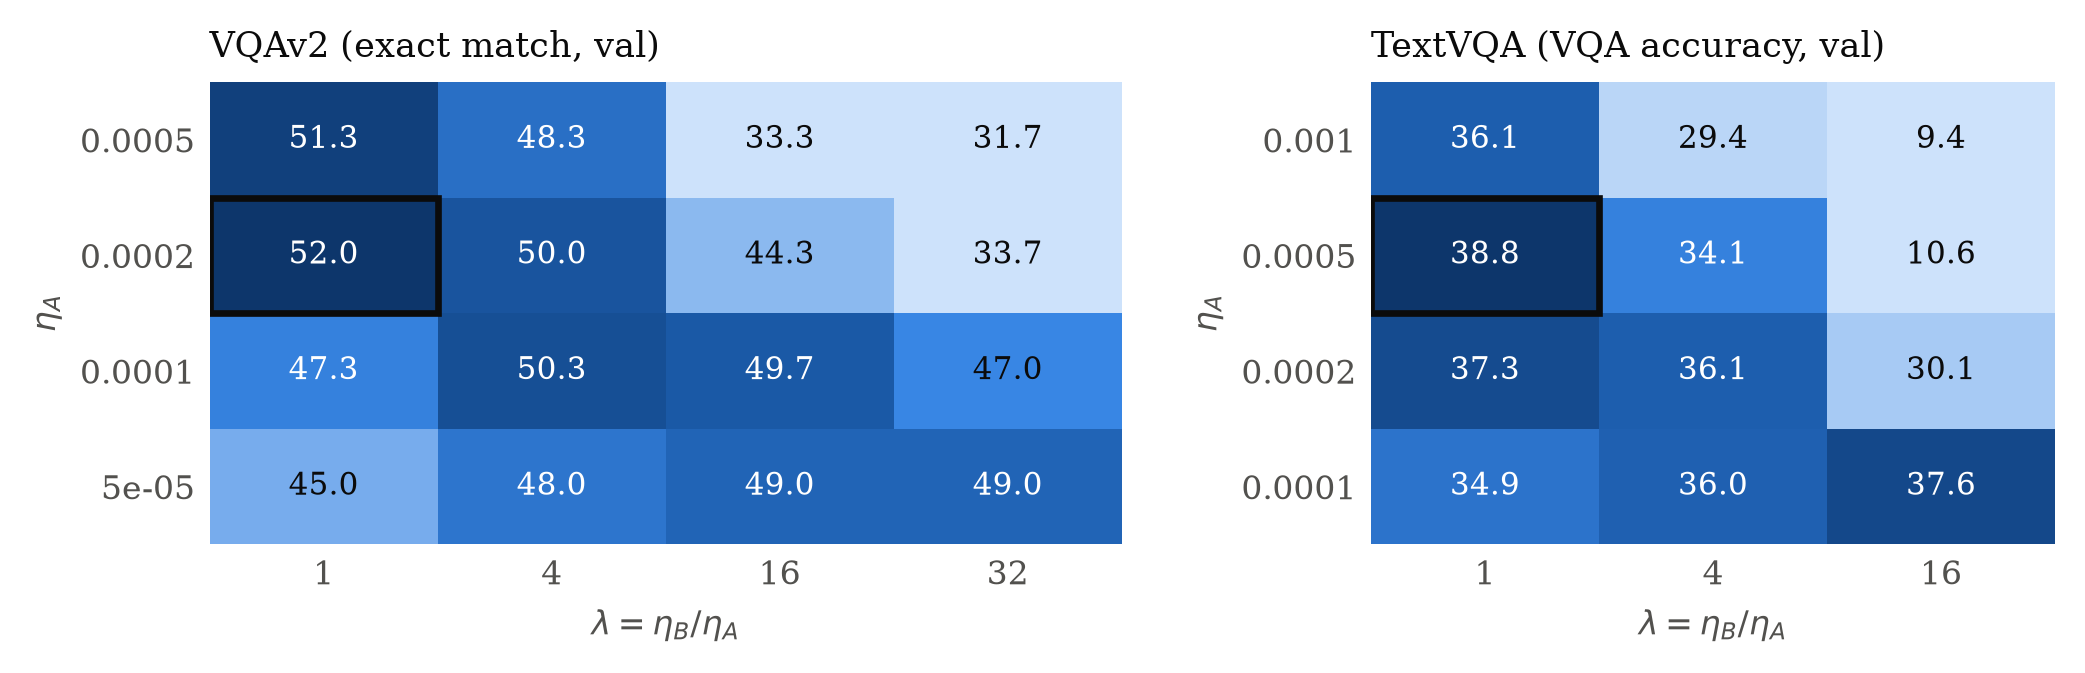
\includegraphics[width=0.94\linewidth]{fig_grid.png}
  \caption{\textbf{H1.} Val accuracy (\%) over $(\etaA, \lambda)$, one seed. The outlined cell is the best. On both
  tasks the optimum lies on the diagonal ($\lambda = 1$, i.e.\ tuned LoRA). $\lambda > 1$ helps only along the
  bottom rows, where $\etaA$ is too small, and collapses training at large $\etaA$.}
  \label{fig:grid}
\end{figure}

\begin{table}[t]
  \centering\small
  \caption{\textbf{Baseline vs.\ adapted (H2).} Test accuracy, mean $\pm$ std over 3 seeds. Speed: seeds that
  reach 95\% of tuned LoRA's final val accuracy (Acc$_{95}$) or its final val loss (Loss), with the median step
  where at least half the seeds reach it. Settings $(\etaA,\lambda)$, VQAv2 / TextVQA: LoRA (2e-4, 1) / (5e-4, 1);
  LoRA+ (1e-4, 4) / (1e-4, 16); drop-in (2e-4, 16) / (5e-4, 16).}
  \label{tab:main}
  \begin{tabular}{@{}lcccccc@{}}
    \toprule
    & \multicolumn{3}{c}{VQAv2 (exact match)} & \multicolumn{3}{c}{TextVQA (VQA acc.)} \\
    \cmidrule(lr){2-4}\cmidrule(l){5-7}
    Method & Test acc. & Acc$_{95}$ & Loss & Test acc. & Acc$_{95}$ & Loss \\
    \midrule
    Zero-shot baseline         & 29.4 & -- & -- & 32.7 & -- & -- \\
    LoRA (tuned)               & \textbf{54.3} $\pm$ 0.7 & 3/3, 188 & 3/3, 296 & \textbf{43.0} $\pm$ 1.5 & 3/3, 469 & 2/3, 592 \\
    LoRA+ (tuned)              & 53.5 $\pm$ 0.5 & 3/3, 281 & 3/3, 296 & 41.3 $\pm$ 0.1 & 1/3 & 0/3 \\
    LoRA+ drop-in $\lambda=16$ & 37.1 $\pm$ 6.2 & 0/3 & 0/3 & 11.2 $\pm$ 0.5 & 0/3 & 0/3 \\
    \bottomrule
  \end{tabular}
\end{table}

\textbf{Baseline vs.\ adapted.} LoRA fine-tuning clearly works. Test accuracy rises from 29.4 to 54.3 on VQAv2 and
from 32.7 to 43.0 on TextVQA (Table~\ref{tab:main}). On VQAv2, part of the gain is answer format: the zero-shot model
scores only 16.9\% on yes/no questions because it often replies with a phrase (``special occasion'') rather than
yes or no.

\textbf{H1 is not supported} (Fig.~\ref{fig:grid}). The best cell is $\lambda = 1$ on both tasks (52.0 vs.\ 50.3 for
the best $\lambda > 1$ on VQAv2; 38.8 vs.\ 37.6 on TextVQA). The grid shows what $\lambda$ actually does at this scale:
at small $\etaA$ it raises accuracy (VQAv2 $\etaA = 5\mathrm{e}{-5}$: $45.0\to49.0$; TextVQA $\etaA = 1\mathrm{e}{-4}$:
$34.9\to37.6$), but tuning LoRA's single learning rate recovers the same gain. In other words, $\lambda$ compensates
for a learning rate that is too small rather than unlocking a better optimum. With one seed and 300 val questions,
gaps of $\lesssim$2 points are within noise, so H1 is \emph{not supported} rather than refuted.

\textbf{H2a and H2b are not supported} (Table~\ref{tab:main}). Tuned LoRA+ is 0.8 (VQAv2) and 1.7 (TextVQA) points
\emph{below} tuned LoRA. On VQAv2 the speed medians differ by at most one checkpoint interval, so there is no
evidence of a speed-up. On TextVQA, LoRA+ reaches 95\% of LoRA's accuracy in 1 of 3 seeds (LoRA: 3 of 3) and never
reaches its val loss. The cleanest comparison holds $\etaA = 10^{-4}$ fixed (tower ablation, 3 seeds): $\lambda=16$
gives $40.8\pm1.6$ test against $45.0\pm0.2$ for $\lambda=1$ (val 37.7 vs.\ 38.9). The same runs show that test
gaps of $\sim$2 points between learning rates are not reliable here: $\eta=10^{-4}$ beats the selected
$5\cdot10^{-4}$ on test (45.0 vs.\ 43.0) but loses on val (38.9 vs.\ 41.0). Using the paper's $\lambda = 16$
without retuning is harmful: it is unstable on VQAv2 and collapses below zero-shot on TextVQA.

\begin{figure}[t]
  \centering
  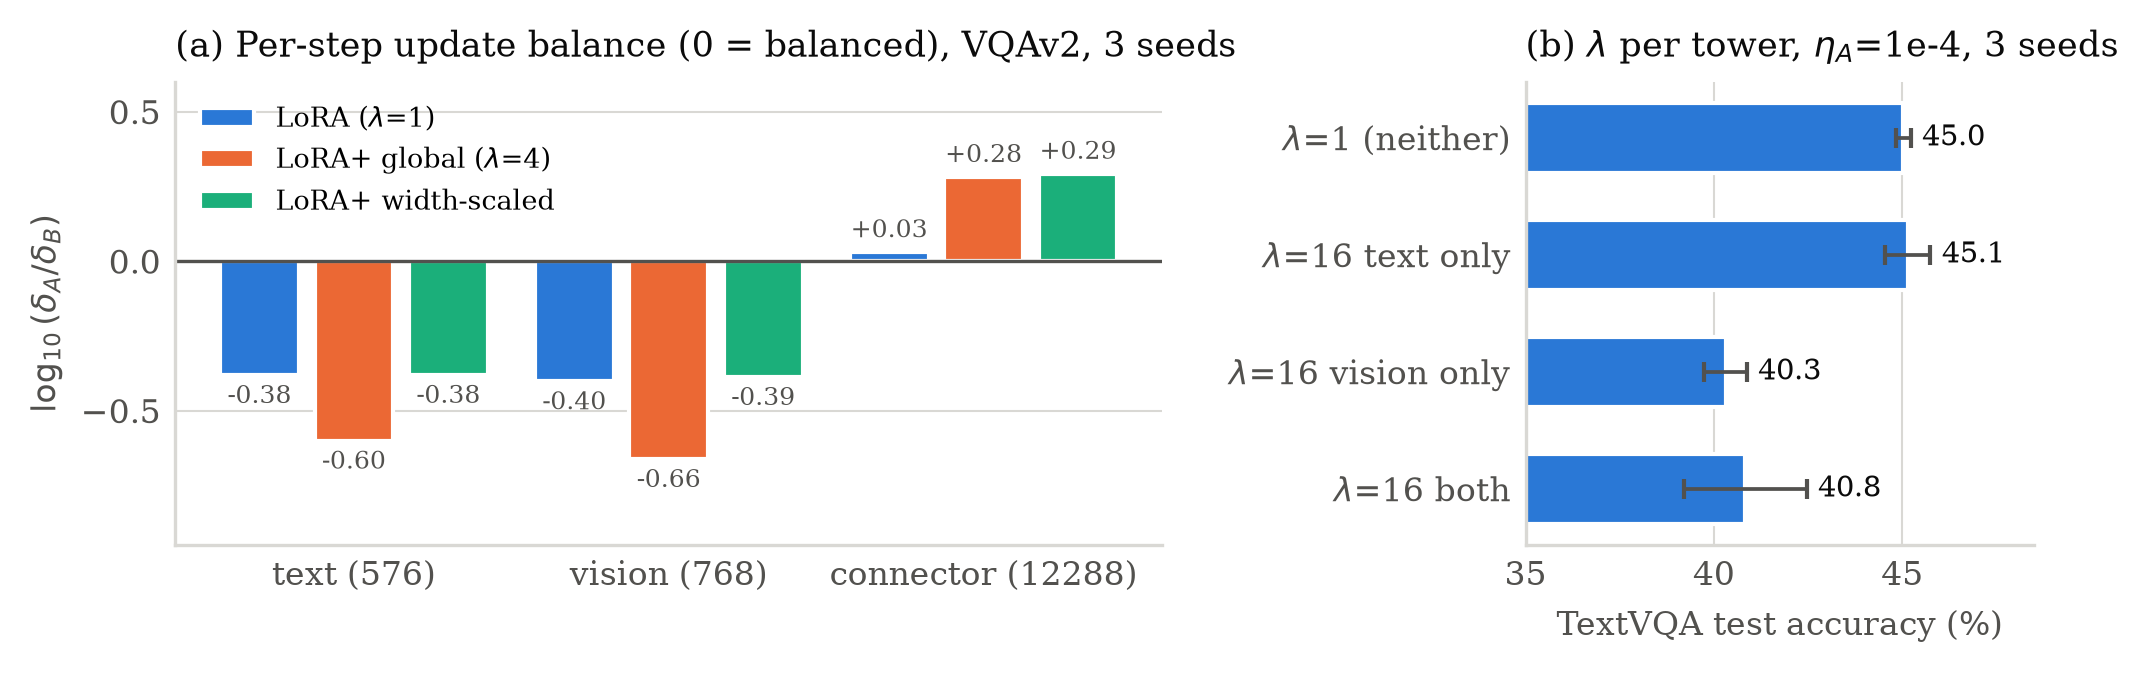
\includegraphics[width=0.97\linewidth]{fig_mechanism.png}
  \caption{\textbf{(a) H3 / bonus:} median $\log_{10}(\delta_A/\delta_B)$ over the second half of training, per
  tower (fan-in in brackets), VQAv2, connector experiment (connector adapted), 3 seeds. \textbf{(b) Tower
  ablation} on TextVQA: $\lambda = 16$ applied to the $B$ matrices of neither, one or both towers, all at
  $\etaA = 10^{-4}$; mean $\pm$ std over 3 seeds.}
  \label{fig:mech}
\end{figure}

\textbf{H3 is not supported, and the mechanism explains the failure} (Fig.~\ref{fig:mech}a). Under plain LoRA,
$\delta_A$ and $\delta_B$ are within a factor of 2.5--5 of each other in the text and vision towers
($\log_{10}(\delta_A/\delta_B)\approx-0.4$ on VQAv2, $-0.7$ on TextVQA): there is no order-of-magnitude imbalance to
correct. Moreover, the sign is the \emph{opposite} of the prediction. With equal learning rates and $B_0=0$, the
paper predicts that $B$ is under-updated ($\delta_B < \delta_A$); we find $\delta_B > \delta_A$. Raising $\etaB$
(global LoRA+) therefore moves the balance further from 1 ($-0.6$). The weight-space view agrees: the share of $\Delta W$ that comes from
$A$ learning, $\|B(A-A_0)\| / (\|BA_0\| + \|B(A-A_0)\|)$, drops from 0.24 to 0.12 on VQAv2 (0.38 to 0.10 on
TextVQA). LoRA+ does shift the update towards $B$, as the theory intends, but there was no deficit to fix. The
analysis in~\cite{loraplus} is explicitly asymptotic (all orders are $\Theta(\cdot)$ in width $n$ as $n \to \infty$;
App.~A.1), so it prescribes how the optimal ratio should \emph{scale} with width, not its value at a given width. Our
measurement shows that at $n = 576$--$768$ the predicted imbalance is not yet present; this does not contradict the
theory, but it limits its practical reach for small VLMs.

\textbf{H4 is not supported.} On the harder TextVQA task, LoRA+ still loses. By question type, LoRA+ minus LoRA is
$-1.5$ (yes/no), $-1.0$ (number) and $-0.2$ (other) on VQAv2, and $-2.9$ (answer appears in the OCR tokens) and
$-0.8$ (answer not in the OCR tokens) on TextVQA. There is no pattern of larger gains on harder questions.

\textbf{Further experiment 1: width-scaled $\lambda$ on the VLM connector is not supported.} We also adapted the 12288-wide
connector (3 seeds, VQAv2). Width-scaled $\lambda$ (connector $\lambda \approx 21$, vision MLP $\lambda \approx 5$)
reached $53.2\pm0.6$, global LoRA+ $53.3\pm0.8$ and plain LoRA $54.5\pm0.3$; width-scaled was also the slowest (370
vs.\ 296 steps). The connector is the only part of the model where $\delta_A \gtrsim \delta_B$ under LoRA (+0.03,
against $-0.4$ elsewhere). This is the direction the width argument predicts, but the effect is far smaller than
the $21\times$ that $\Theta(\text{fan-in})$ scaling implies, so scaling $\lambda$ by fan-in overshoots.

\textbf{Further experiment 2: the vision encoder is the part that does not tolerate a large $\etaB$} (Fig.~\ref{fig:mech}b). A
$2\times2$ ablation on TextVQA (3 seeds, all at $\etaA = 10^{-4}$) applies $\lambda = 16$ to the decoder, the
encoder, both or neither. Paired by seed, the main effect of $\lambda$ in the \textbf{vision encoder} is
$\mathbf{-4.5\pm0.6}$ points (negative in every seed: $-4.5$, $-5.3$, $-3.8$). In the language decoder it is
$+0.3\pm1.0$, and the interaction is $+0.4\pm2.5$, i.e.\ none. A global $\lambda$, as LoRA+ prescribes, therefore
applies a large $\etaB$ to the encoder whose fine-grained features OCR-style VQA depends on. This is a constraint a
text-only study cannot reveal. It is also the \emph{opposite} of the width prediction, since the vision tower is the
wider of the two.

\textbf{Conclusion.} The LoRA+ claim does \textbf{not} transfer to SmolVLM-256M on VQAv2 or TextVQA. A tuned LoRA
learning rate matches or beats LoRA+ in accuracy and speed. The paper's mechanism explains why: at these widths,
plain LoRA's update terms are already close to balanced, with $B$ slightly ahead rather than behind. In the VLM
setting, the large $B$ learning rate hurts the vision encoder specifically ($-4.5\pm0.6$ points), and scaling
$\lambda$ by layer width does not fix it. \textbf{Limitations:} one model size; a single-seed grid run at a shorter
budget than the final runs; exact-match accuracy and a question-level (not image-level) split on VQAv2; test gaps of
$\sim$2 points are within split noise; re-running the same seed varies by $\approx$1 point due to GPU
non-determinism. \textbf{Code:} \texttt{part1/part1\_loraplus\_smolvlm.py} runs every experiment
(\texttt{--experiment \{main,delta,connector,tower\}}); \texttt{--experiment single} retrains one main-table run from
scratch, and \texttt{part1/colab\_reproduce\_part1.ipynb} does so on a Colab T4 (see \texttt{part1/README.md}).

\vspace{-4pt}
{\small
\begin{thebibliography}{9}\setlength{\itemsep}{0pt}
\bibitem{loraplus} S.~Hayou, N.~Ghosh, B.~Yu. LoRA+: Efficient low rank adaptation of large models. arXiv:2402.12354, 2024.
\bibitem{lora} E.~J.~Hu et al. LoRA: Low-rank adaptation of large language models. ICLR, 2022.
\bibitem{smolvlm} A.~Marafioti et al. SmolVLM: Redefining small and efficient multimodal models. arXiv:2504.05299, 2025.
\bibitem{vqav2} Y.~Goyal et al. Making the V in VQA matter. CVPR, 2017.
\bibitem{textvqa} A.~Singh et al. Towards VQA models that can read. CVPR, 2019.
\end{thebibliography}}
\end{document}
